% Chapter Template

\chapter{Results and Discussion} % Main chapter title

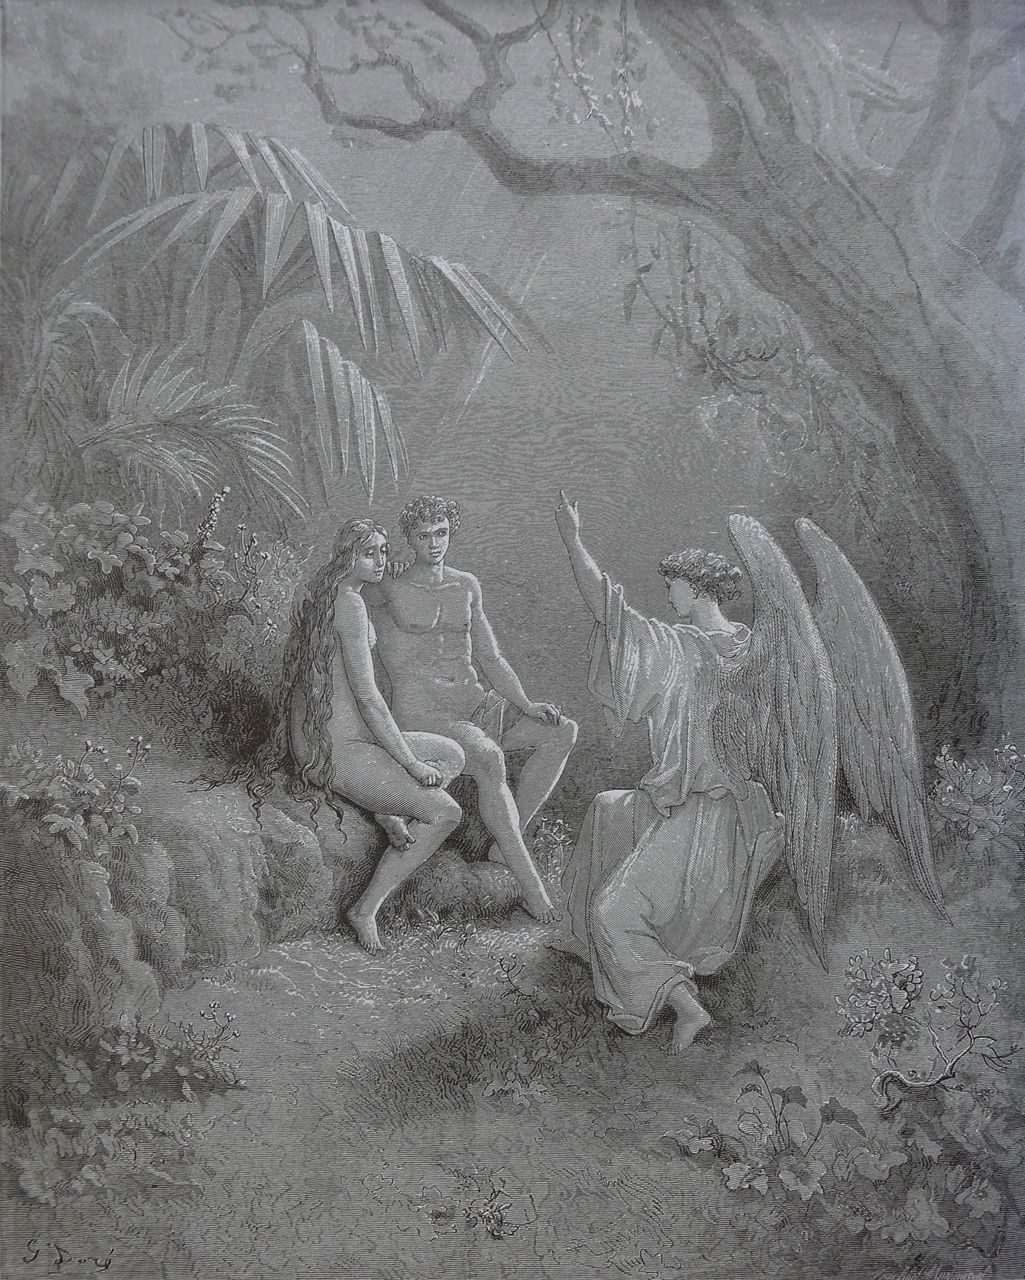
\includegraphics[width=\linewidth,trim={0 7cm 0 12cm},clip]{Paradise_Lost_22}

\label{Chapter 7} % Change X to a consecutive number; for referencing this chapter elsewhere, use \ref{ChapterX}

%----------------------------------------------------------------------------------------
%	SECTION 1
%----------------------------------------------------------------------------------------
%% Look back at what was achieved and comment on the research questions. How they were answered, fully yes fully no, partially?

\section{Matrix Mode Operation}


%-----------------------------------
%	SUBSECTION 1
%-----------------------------------
\subsection{Subsection 1}


%----------------------------------------------------------------------------------------
%	SECTION 2
%----------------------------------------------------------------------------------------

\section{Secure Compartment Implementation}

%----------------------------------------------------------------------------------------
%	SECTION 3
%----------------------------------------------------------------------------------------

\section{Research Question Satisfaction}

\textit{What are the missing or non-functional sub-systems that the MEGA65 requires to be implemented?}\\
Over the course of the project, several missing and/or non-functional sub-systems were found within the MEGA65 smart phone. Of those sub-systems, the ones that were fixed are detailed in the previous chapters of this document. Desipte the fixes applied, there are still many sub-systems of the phone that require additional attention in order for them to function as intended.\\
One of the functions of the phone is being able to create and load save states that are images of the phone at a particular point in time. These save states are mostly function, but there are still some strange cases, in which, their function causes issues for the user. It was noted, but not explored, that creating a save state in the most recent version of the phone causes the partition table to be invalidated. This is suspected to be the result of some change to the save state code causing the slot pointer to point to the partition table instead of the desired slot.\\
The save state error also has a cascading effect into the implementation of secure mode, as discussed in chapter \ref{Chapter 6}. As described in section \ref{Ch6 Sec3 Sub2}, the secure mode implementation planns to use this save state proccess as a part of it, this error will therefore cause the secure state to corrupt the patition table.\\
In addition to the partition corrupting, the secure mode is also non-functional for a number of other reasons. The string comparison seen in figure \ref{fig:monitoracceptreject}, only compares the input to the upper case version of accept or reject. While this could be intentional to ensure that the user truely desires the result, by entering reject in lower case an instruction is invoked. This is due to the lower case r character being an instructional prefix. Another issue with secure mode is when successfully rejection secure compartments, when the SD card has been removed from the device there is currently no protection against reloading. This causes the secure mode to load from nothing and produces unpredictable results.\\
Although functionality to matrix mode has mostly been restored, it is not working entirely as intended. From within matrix mode it is possible to halt and single step the CPU, if the CPU is halted, then a request to leave matrix mode is send and stepped through, the user is left in user mode with a frozen CPU and no way to return to matrix mode.
When exiting from matrix mode with the secondary exit keycode, superkey + ~, the ~ key is printed in user mode. This is believed to be due to double scanning of the non-special input keys.\\
When experimenting with the SD card compatability, it was noted that the SDXC card was not recognised as an SD card at all. Investigation into the SD card hardware showed that there was no case for this type of card. In addition to this, in the latest version of the phone, the SD card detecion no longer recans for the SD card if one is not initially detected.\\
\\
\textit{How can these sub-systems be implemented?}\\
\begin{itemize}
\item{Load and Save Sate}\\
  The save state partition table corruption issue should be solved by reviewing the location at which the save state is attemping to be saved to. This location should be confimred as save state slot. Additionally, the size of the data being saved should be compared to the size of the save state slot to ensure that other data is not being overwritten.
\item{ACCEPT/REJECT Strings}\\
  To ensure the secure compartment sub-system is functional and in accordance with the user's expectations, the lower case versions of accept and reject should also have the same functionality as the upper case versions. Conversely to this, if the accept and reject cases are restricted to upper case only, inputing a lower case version should send a warning to the user and, in the reject case, not throw a syntax error.
\item{CPU Locking}\\
  To prevent CPU locking and restore some functionality to matrix mode, exiting matrix mode should be tied into unfreezing the CPU.
\item{SD card Protection}\\
  To protect the SD card against loading junk data from the SD card slot when the SD card is removed a fail state should be implemented when the attempting to load and no SD card is detected. This state should prompt the user to insert an SD card and specify the slot they wish to load from.
\item{SDXC Support}\\
  The SDXC SD cards should have their data sheet evaluated and the functionality required to used them added to the SD card handeling hardware.
\end{itemize}

\textit{How can the simplicity, understandability and hence, the security of these sub-systems be maximised?}\\
blah
\\
\textit{How can the complete MEGA65 architecture be physically prototyped on the bench?}\\
blah
\\
\textit{How can the secure compartmentalisation's architecture planned for the MEGA65 be realised?}\\
blah
\\


%----------------------------------------------------------------------------------------
%	SECTION 2
%----------------------------------------------------------------------------------------

\section{Future Work}
